\documentclass[tikz,border=10pt]{standalone}
\usepackage{tikz}
\usetikzlibrary{shapes,arrows,positioning,calc,shadows}

\begin{document}

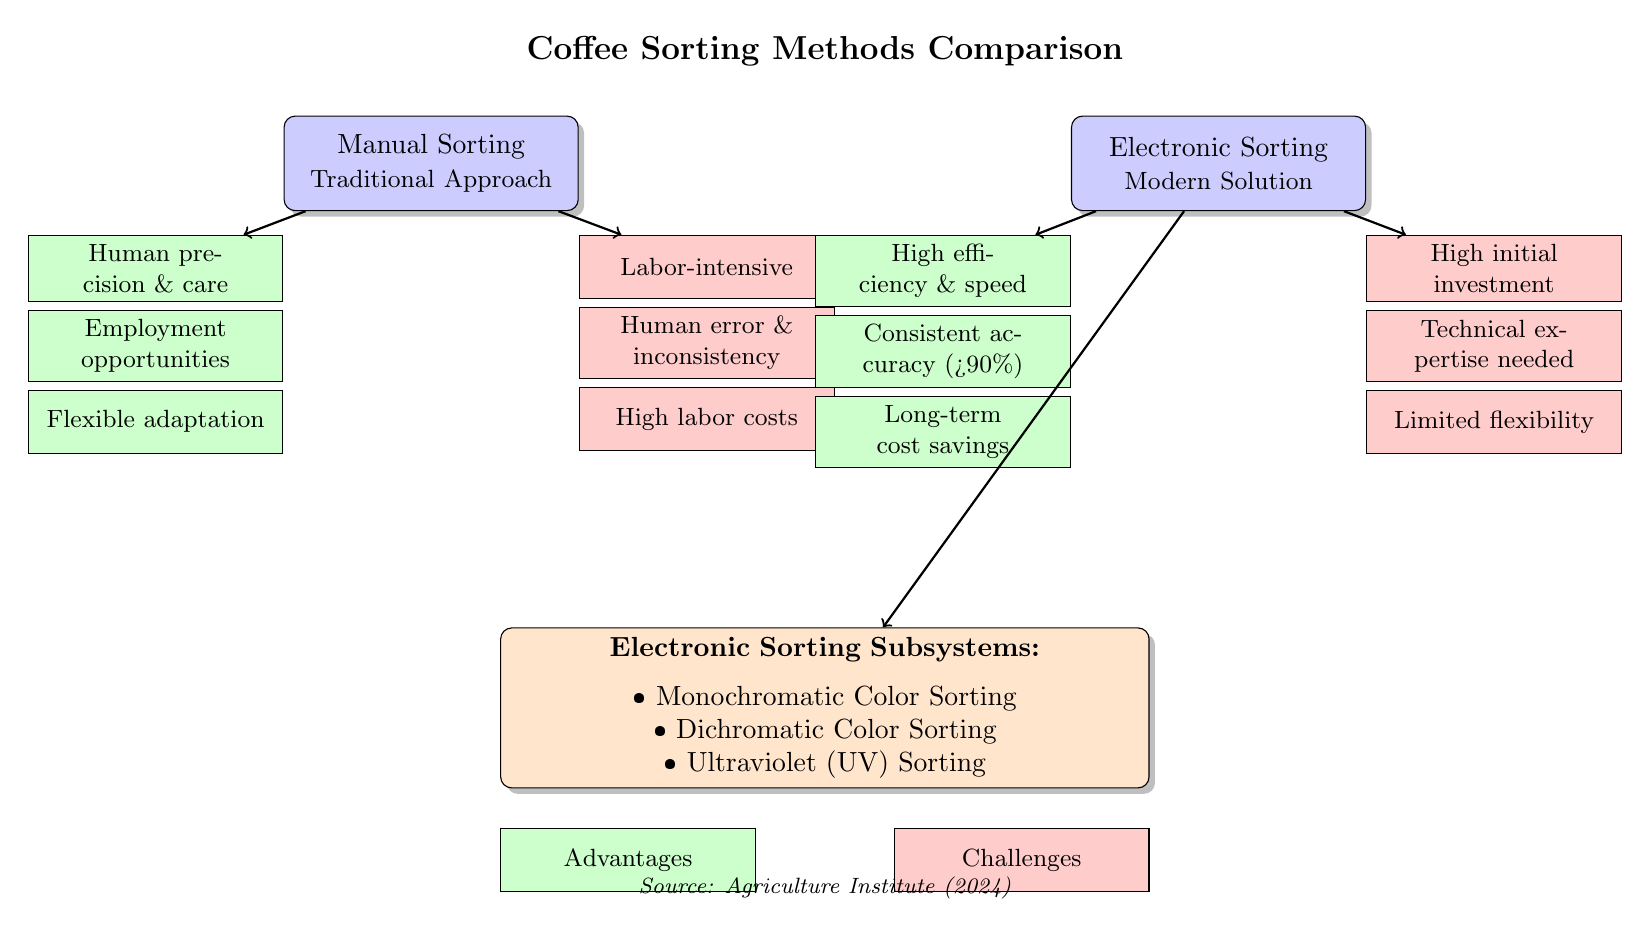
\begin{tikzpicture}[
    node distance=2cm,
    method/.style={rectangle, draw, fill=blue!20, text width=3.5cm, text centered, rounded corners, minimum height=1.2cm, drop shadow},
    advantage/.style={rectangle, draw, fill=green!20, text width=3cm, text centered, minimum height=0.8cm, font=\small},
    challenge/.style={rectangle, draw, fill=red!20, text width=3cm, text centered, minimum height=0.8cm, font=\small},
    title/.style={font=\bfseries\large}
]

% Title
\node[title] (title) {Coffee Sorting Methods Comparison};

% Manual Sorting Section
\node[method, below=0.5cm of title, xshift=-5cm] (manual) {Manual Sorting\\{\small Traditional Approach}};

\node[advantage, below=0.3cm of manual, xshift=-3.5cm] (ma1) {Human precision \& care};
\node[advantage, below=0.1cm of ma1] (ma2) {Employment opportunities};
\node[advantage, below=0.1cm of ma2] (ma3) {Flexible adaptation};

\node[challenge, below=0.3cm of manual, xshift=3.5cm] (mc1) {Labor-intensive};
\node[challenge, below=0.1cm of mc1] (mc2) {Human error \& inconsistency};
\node[challenge, below=0.1cm of mc2] (mc3) {High labor costs};

% Electronic Sorting Section
\node[method, below=0.5cm of title, xshift=5cm] (electronic) {Electronic Sorting\\{\small Modern Solution}};

\node[advantage, below=0.3cm of electronic, xshift=-3.5cm] (ea1) {High efficiency \& speed};
\node[advantage, below=0.1cm of ea1] (ea2) {Consistent accuracy (>90\%)};
\node[advantage, below=0.1cm of ea2] (ea3) {Long-term cost savings};

\node[challenge, below=0.3cm of electronic, xshift=3.5cm] (ec1) {High initial investment};
\node[challenge, below=0.1cm of ec1] (ec2) {Technical expertise needed};
\node[challenge, below=0.1cm of ec2] (ec3) {Limited flexibility};

% Subsystems box
\node[method, below=7cm of title, fill=orange!20, text width=8cm] (subsystems) {
    \textbf{Electronic Sorting Subsystems:}\\[0.2cm]
    • Monochromatic Color Sorting\\
    • Dichromatic Color Sorting\\
    • Ultraviolet (UV) Sorting
};

% Connect lines
\draw[->, thick] (manual) -- (ma1);
\draw[->, thick] (manual) -- (mc1);
\draw[->, thick] (electronic) -- (ea1);
\draw[->, thick] (electronic) -- (ec1);
\draw[->, thick] (electronic) -- (subsystems);

% Legend
\node[advantage, below=0.5cm of subsystems, xshift=-2.5cm] (leg1) {Advantages};
\node[challenge, below=0.5cm of subsystems, xshift=2.5cm] (leg2) {Challenges};

% Source citation
\node[below=1cm of subsystems, font=\footnotesize\itshape] (source) {Source: Agriculture Institute (2024)};

\end{tikzpicture}

\end{document}
